\documentclass[twocolumn,12pt]{article}
	
	
	\usepackage{url}
	\usepackage{hyperref}
	\usepackage{graphicx}

\newcommand{\brand}[1]{\textit{#1}}

\title{\brand{Jellypanel}}

\begin{document}
	
	\maketitle
	
	

	\tableofcontents
	\listoffigures
	
	Recentemente, a \href{https://www.google.com.br/}{\brand{Google}} anunciou que irá descontinuar o \href{https://jamboard.google.com/}{\brand{Jamboard}}\footnote{\url{https://support.google.com/jamboard/answer/14084927}} (Figura~\ref{fig:gmail}). 
	Os aplicativos e quadros digitais precisarão, então, de substitutos.
	O próprio \brand{Google} recomenda produtos seus parceiros, como  \brand{Figma}\footnote{\url{https://www.figma.com/figjam/jamboard-alternative/}}, \brand{Lucid}\footnote{\url{https://lucid.co/compare/jamboard-replacement}} e \brand{Miro}\footnote{\url{https://miro.com/migrate-from-jamboard/}}.   				
	Esse mercado é o objetivo deste trabalho. 
	
	\begin{figure}[htpb]
		\caption{E-mail de desativação do \brand{Jamboard}}
		\label{fig:gmail}
		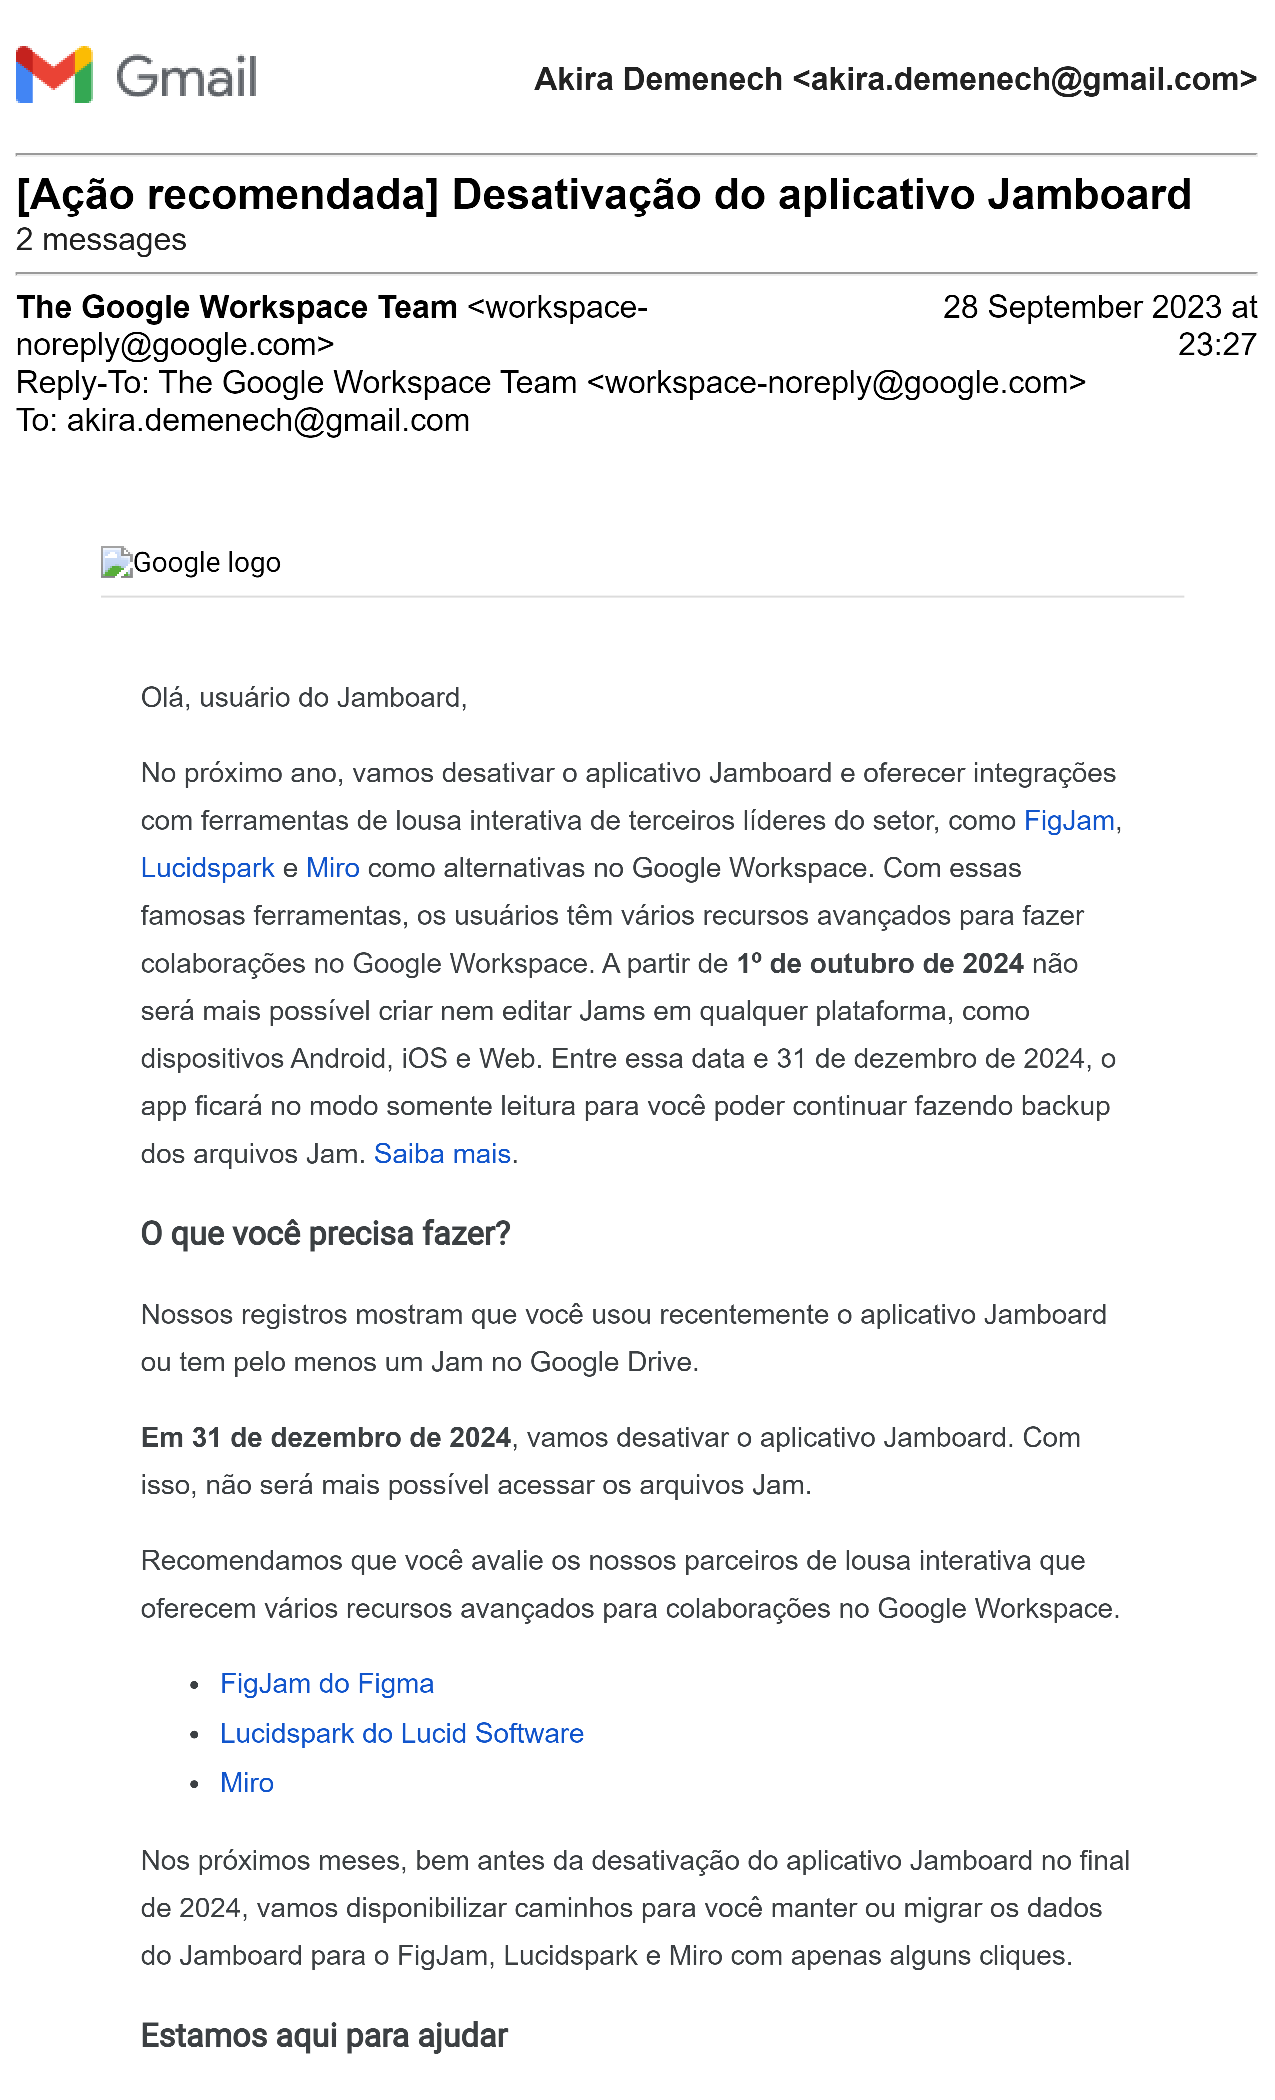
\includegraphics[width=\linewidth]{jamboard.pdf}
	\end{figure}

	
	

\end{document}
